\documentclass[10pt,journal]{IEEEtran}

\usepackage[scale=0.8]{geometry}
\usepackage{graphicx}

% This centers the captions
\makeatletter
\long\def\@makecaption#1#2{\ifx\@captype\@IEEEtablestring
\footnotesize\begin{center}{\normalfont\footnotesize #1}
{\normalfont\footnotesize\scshape #2}\end{center}
\@IEEEtablecaptionsepspace
\else
\@IEEEfigurecaptionsepspace
\setbox\@tempboxa\hbox{\normalfont\footnotesize {#1.}~~ #2}
\ifdim \wd\@tempboxa >\hsize
\setbox\@tempboxa\hbox{\normalfont\footnotesize {#1.}~~ }
\parbox[t]{\hsize}{\normalfont\footnotesize \noindent\unhbox\@tempboxa#2}
\else
\hbox to\hsize{\normalfont\footnotesize\hfil\box\@tempboxa\hfil}\fi\fi}
\makeatother

\title{Design and implementation of the $sin$ function for an 8-bit MIPS processor}
\author{Dominik Laskowski, Payom Meshgin, Daniel Ranga, Ming Yang}

\begin{document}
\maketitle

\section{Motivation / Background}
Hardware acceleration of transcendental functions is crucial for real-time systems
performing computationally intensive tasks like computer graphics and audio processing.
The x87 floating-point unit in the IA-32 architecture supports instructions like \texttt{fsin}
and \texttt{fsincos}. Likewise, graphics processing units and digital signal processors
provide dedicated logic for trigonometric operations.

Lookup tables based on ROMs and PLAs are the most common approach for implementing $sin$
in hardware. They are often coupled with approximation techniques like interpolation to
achieve adequate precision while reducing transistor count. An alternative method that
offers better precision at the expense of speed is the Taylor series expansion. Finally,
the CORDIC (for Coordinate Rotation Digital Computer) algorithm is desirable in embedded
systems without a multiplier, since it only requires adders, shifters and lookup tables.
In this report, we investigate the design and implementation of a $sin$ functional block for
an 8-bit MIPS processor, using the first two aforementioned approaches.

In practice, $sin$ blocks usually operate on 32-bit IEEE 754 floating-point numbers. However,
since the MIPS core has 8-bit registers and integer operations only, we opted for a custom encoding
scheme based on binary scaling. The assumed domain and image is $[0, \frac{\pi}{2}]$ and $[0, 1]$,
respectively. These ranges are discretized to an integer between $0$ and $255$.

\section{Design Implementation}
\subsection{Lookup Table Implementation}
The $sin$ lookup table is a NOR-NOR PLA with 8-bit input and output. The design process for this
implementation was straightforward. The decimal and binary representations of the 256 angles and
$sin$ results were calculated in an Excel spreadsheet and exported to a CSV file. A simple Python
script was written to convert the CSV file into a Verilog \texttt{casez} statement. The schematic
and layout, shown in Figure \ref{lut}, were obtained from the PLA generator and tweaked in Electric
to pass DRC. Figure \ref{mips_lut} is the final layout after the lookup table was mirrored vertically
and wired up to the datapath.

\begin{figure}[h]
\centering
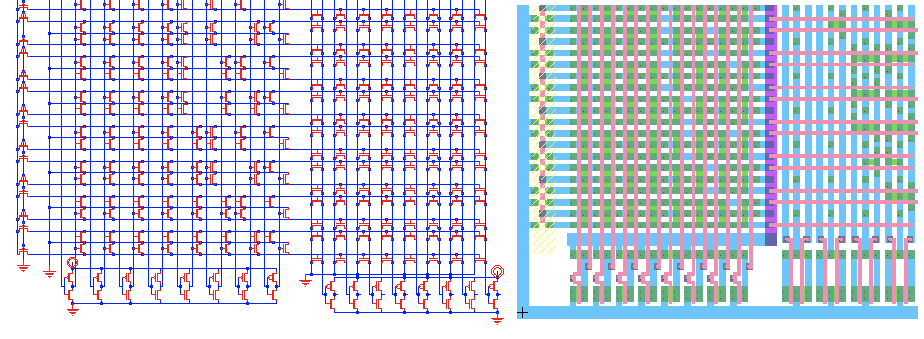
\includegraphics[width=3in]{lut.png}
\caption{Schematic and layout of the lookup table}
\label{lut}
\end{figure}

\begin{figure}[h]
\centering
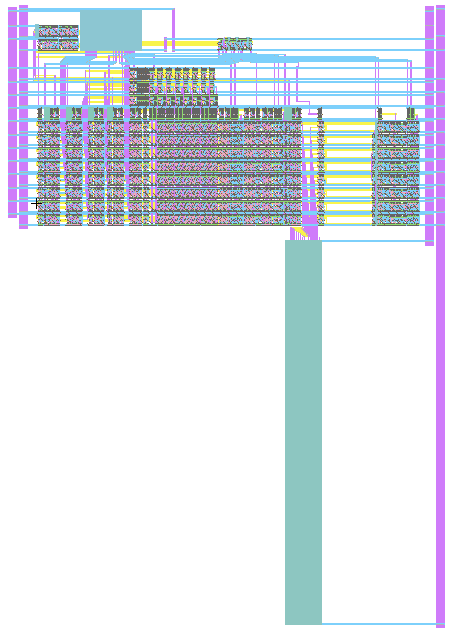
\includegraphics[width=3in]{mips_lut.png}
\caption{Layout of MIPS core with lookup table}
\label{mips_lut}
\end{figure}

\subsection{Taylor expansion design}
\begin{equation}
\label{sin-taylor}
sin(x) = x - \frac{x^3}{3!} + \frac{x^5}{5!}+ O(x^7)
\end{equation}

\begin{figure}[h]
\centering
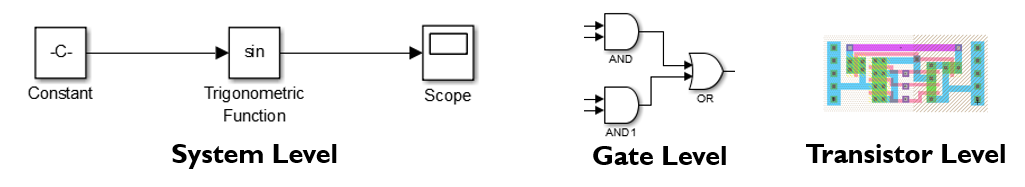
\includegraphics[width=3in]{design_methodology.png}
\caption{Circuit Design Methodology}
\label{design_methodology}
\end{figure}

The formula written in equation \ref{sin-taylor} is a three-term expansion of Taylor series for $sin(x)$. In this project, we implemented a combinational logic circuit based on this equation to evaluate the $sin$ function. The reason for choosing that is related to the goal of this project, which is to have a $sin$ function generator with an accuracy that is comparable to the LUT solution, and Taylor series does provide an adjustable accuracy, based on the number of terms included the evaluation.

During the design phase of this circuit, as shown in Fig.\ref{design_methodology}, a top-to-down design approach is followed to implement system-level, gate-level and transistor level design of the entire system. More specifically, due to the fact that the same interface is used for circuit design and simulation in Simulink, circuit design becomes much more efficient than the case that it is designed in Electric and then get verified in ModelSim. Therefore, the system-level and gate level design and simulation are both implemented in Simulink, and then they are directly translated into Electric to implement the transistor-level design after the gate-level design functionality has been verified. 

\begin{figure}[h]
\centering
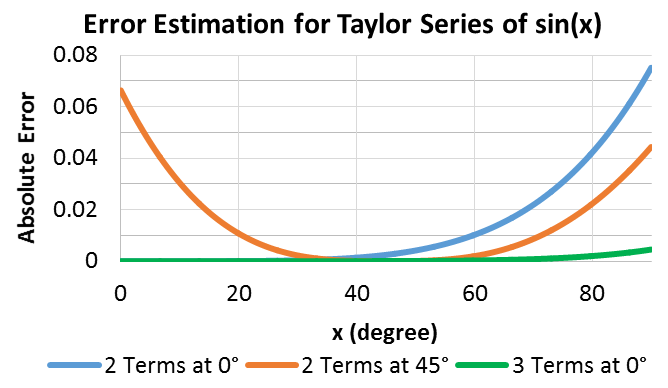
\includegraphics[width=3in]{error-estimation.png}
\caption{Absolute approximation error with different Taylor series}
\label{error-estimation}
\end{figure}

At the beginning of the project, an error estimation process is conducted to help us identify the target of this design so that the corresponding circuit can be build up based on specific design requirements. Fig.\ref{error-estimation} demonstrates the absolute approximation error caused by applying Taylor series with different conditions. Since the design is required to have similar accuracy as the LUT implementation (error ≤0.2\%), we decided to use three terms Taylor series and expand it respect to zero so that the estimation error is ensured to be smaller than 0.5\%.

\begin{figure}[h]
\centering
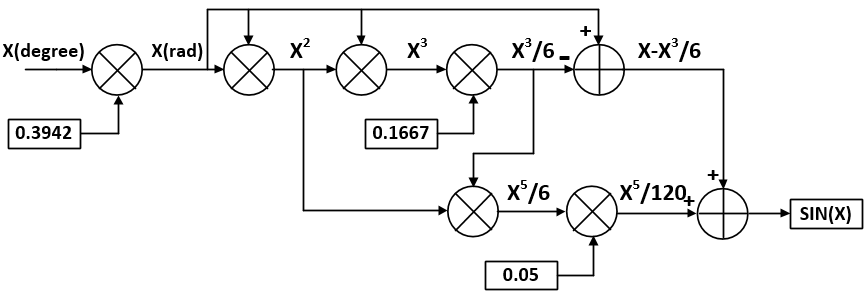
\includegraphics[width=3in]{finalized_design.png}
\caption{Finalized system-level design of Taylor series implementation}
\label{finalized_design}
\end{figure}

Fig.\ref{finalized_design} illustrates the finalized system-level implementation of Taylor series implementation and several optimizations have been made at this level. First of all, some of the generated numbers, such like $x^2$ and $x^3/6$, can be reused in this algorithm to reduce the complexity of the circuit. Second, division can be carried out by multipliers since the dividend is always larger than one. The cost can be further reduced by shifting operation if the dividend contains a factor of 2. To make the design consistent with our loop-up table implementation, we were about to encode all the floating point numbers by shifting 8 bits in our system. However, it turns out that this will lead to an error if the input value becomes larger than 1 in radians degrees). Therefore, as demonstrated in the figure, a multiplier is placed in the front end of the entire circuit so that the input value can be encoded by shifting 6 bits to the right, and the floating point precision has to be compromised by 2 bits.

\begin{figure}[h]
\centering
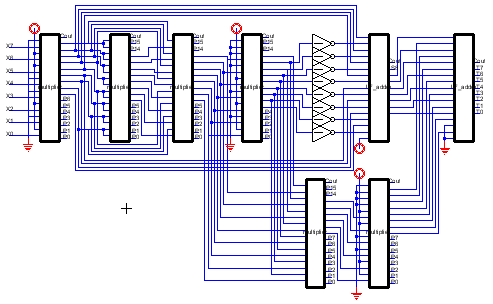
\includegraphics[width=3in]{finalized_gate_design.png}
\caption{Finalized gate-level design of Taylor series implementation}
\label{finalized_gate_design}
\end{figure}

In schematic design, based on the information provided in the textbook, the 8-bits Ladner-Fischer adder and carry-save adder design are performed in the multiplier design to effectively reduce the propagation delay on the critical path. Mirrored version of carry-save adder is also used to improve its shape during the layout process so that it will be in an organized rectangular form. Fig.\ref{finalized_gate_design} shows the finalized gate-level schematic design for the overall system in Electric.

\begin{figure}[h]
\centering
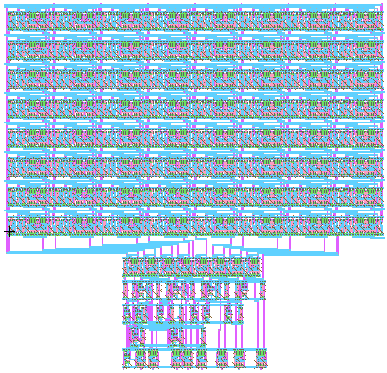
\includegraphics[width=3in]{finalized_transistor_design.png}
\caption{finalized transistor-level layout design of multiplier}
\label{finalized_transistor_design}
\end{figure}


The transistor-level implementation is performed based on the validated schematic design demonstrated in the previous section. Fig.\ref{finalized_transistor_design} illustrates the layout design of the 8-bits multiplier. The carry-save adder section is well organized in a rectangular shape and a LF adder is placed on the bottom to sum up each carry bit. The entire system is organized in a similar way, and because of the correct methodology practiced in this design, the simulation for the system was successful for the first trial.

\subsection{Modification to MIPS processor}

\section{Validation}

	\subsection{Look-up table design}
	\subsection{Taylor expansion design}
	\subsection{Modification to MIPS processor}

\section{Results}

\section{Evaluation}
The two implementations of the design were evaluated using the following three metrics:
\begin{itemize}
\item Accuracy (Error between the output of functional block and the theoretical evaluation of the sine function)
\item Size (Number of transistors in the layout of the functional block)
\item Scalability (How the complexity of the design scales as the bit-width of the signals increase
\end{itemize}

\subsection{Accuracy}
\subsection{Size}
\subsection{Scalability}

\section{Possible improvements}


\section{Conclusion}

\end{document}
